%! TEX root = ../main.tex
% ==============================================================
% IMMUTABLE — generated automatically, do not edit this block
%
% — Provenance ───────────────────────────────────────────────────
%   script            : analysis_scratch/wind_qc_3s_thesis.py
%   computed_in       : analysis_scratch/wind_qc_3s.py (per-run σ over first 3 s) → analysis_scratch/wind_qc_3s_thesis.py (thesis render)
%   plot_type         : wind_qc_boxplot
%   data_class        : DELEG
%   generated_at      : 2026-05-01T14:36:43
%   findings_doc      : (none — diagnostic figure, see immutable-block caveats)
%
% — Thesis context ──────────────────────────────────────────────
%   chapter           : 04
%   caption_label     : fig:ch04_wind_qc_boxplot
%   caption_short     : 
%
% — Filters ────────────────────────────────────────────────────
%   panel             : all
%   wind              : full+no+lowest
%   amplitude [V]     : 
%   frequency [Hz]    : 
%   probes            : 
%   run_category      : 
%   quality_flag      : ok
%   mooring           : 
%
% — Data provenance ────────────────────────────────────────────
%   n_runs            : 
%   in_probes_used    : 
%   out_probes_used   : 
%   probe_configs     : 
%   non_final_config_n: 
%   datasets        :
%     (none registered — set plot_utils.ACTIVE_DATASETS)
%   run_paths       :
%     (omitted — aggregate over > threshold runs, see datasets)
%
% — Method / numerical parameters ─────────────────────────────
%   grouper           : 
%   collapse_panels   : 
%   fft_window_hz     : 0.0
%   extra_params      : Each box pools the first-3 s σ_η across all ok runs at one (WindCondition × date) cell. Whiskers: 5-95 percentile; median = solid black line; box = IQR. Long-run reference (grey band + dashed mean) overlaid. Box face colour = wind condition (CLAUDE.md WIND_COLOR_MAP, alpha=0.42). Datasets: canon March-2026 -lowrange. QC caveats. (1) Stratification: snippets are grouped here only by WindCondition × date; other run-level factors (Mooring, PanelCondition, run-type per40/per240, time-of-day, instrument-cable touches) are NOT yet decomposed and may explain part of the within-group scatter — refine before publication. (2) Probe noise floor: OUT (12400/250) σ sits inside the probe's measured stillwater noise envelope (0.14-0.36 mm; gold standard ≈0.14 mm, CLAUDE.md §16). Apparent OUT-side scatter is therefore partly the noise floor of the probe itself, not genuine variability of the wind-wave field. (3) Reference band: long-run σ range drawn from 5 fullwind+nowave runs of 31, 33, 63, 360, 381 s duration (only 2 of 5 are ≥ 360 s); ensemble mean is dashed. 
%
% — Summary stats cited in caption ────────────────────────────
%   stat:long_sigma_mean_mm[9373/170] : 4.281
%   stat:long_sigma_mean_mm[12400/250] : 0.360
%   stat:n_runs_total : 118
%
% — Subfigures available ───────────────────────────────────────
%     FIGURES/ch04_wind_qc_boxplot.pdf
% ── end immutable block ─────────────────────────────────────────
\begin{figure}[htbp]
  \centering
  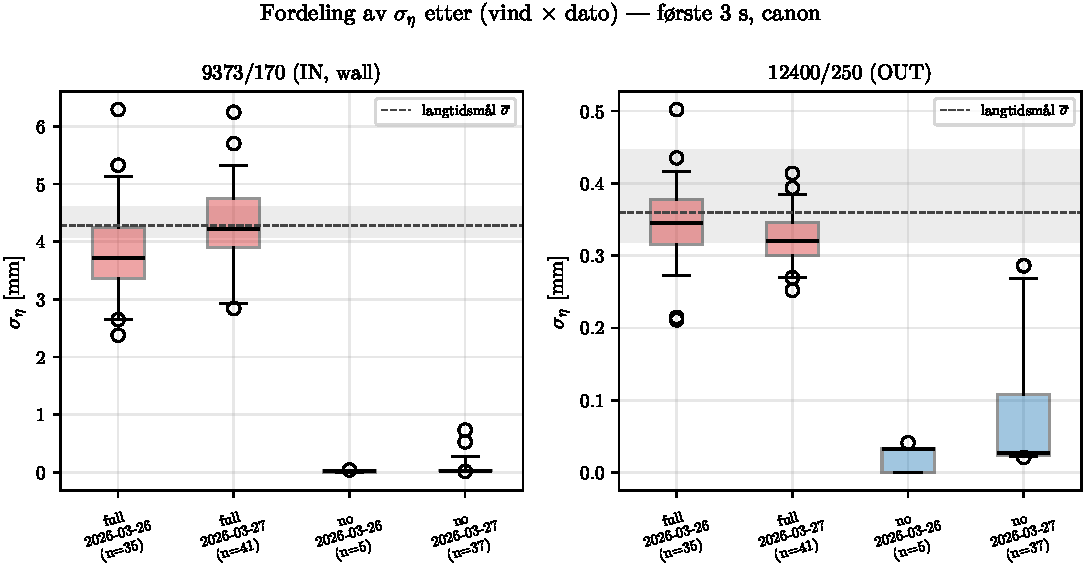
\includegraphics[width=\linewidth]{FIGURES/ch04_wind_qc_boxplot.pdf}
  \caption{
    % TODO: write caption
  }
  \label{fig:ch04_wind_qc_boxplot}
\end{figure}
